\documentclass[9pt,a4paper,twocolumn,twoside]{tau-class/tau}
\usepackage[english]{babel}
\usepackage{booktabs}
\usepackage{tabularx}
\usepackage{array}
\usepackage{graphicx}
\usepackage{float}
\usepackage{caption}
\usepackage{subcaption}
\usepackage{pgfplots}
\usepackage{tikz}
\pgfplotsset{compat=1.18}

\definecolor{tableheader}{HTML}{D9E8FB}
\definecolor{tablerow}{HTML}{F6F9FE}
\definecolor{tableaccent}{HTML}{E8F5E9}
\definecolor{tablewarn}{HTML}{FFF3E0}
\definecolor{tableemph}{HTML}{FCE4EC}
\definecolor{youngcolor}{HTML}{5B8FF9}
\definecolor{adultcolor}{HTML}{61DDAA}
\definecolor{elderlycolor}{HTML}{F6BD16}

\newcolumntype{Y}{>{\raggedright\arraybackslash}X}
\captionsetup[table]{labelformat=simple,labelsep=colon,name=Table}

\doctype{Weekly Lab Report}
\title{Week 10 Report}

\author[a,1]{Yiran Liu\thanks{\href{mailto:yiran.liu@canada.ca}{yiran.liu@canada.ca} (Y. Liu)}}
\affil[a]{NRC - Digital Technology}

\dates{Compiled on \today}
\footinfo{Week 10 Lab Report}
\theday{\today}
\organization{NRC - Digital Technology}
\leadauthor{}

\begin{abstract}
\end{abstract}

\keywords{}

\begin{document}

\maketitle
\thispagestyle{firststyle}

\section{Executive Summary}

Last week, we implemented the conversion pipeline from SMPL mesh to NTU-25 joint format and validated the standalone ST-GCN++ reimplementation against the full NTU RGB+D 120 dataset (82.6\% top-1 accuracy, closely matching the published 83.2\% benchmark). 

This week, two remaining issues in the SMPL$\rightarrow$NTU-25 conversion pipeline were resolved (T-pose contamination and boundary frame padding), and the cleaned Van Criekinge dataset (450 clips, 138 subjects) was verified by running the pretrained action recognition model on the full dataset---achieving 100\% walking-action classification.

With the data pipeline validated, I made a second attempt to fine-tune the ST-GCN++ model with a custom 3-class age classifier (Young $<$40, Adult 40--64, Elderly $\geq$65). However, the initial results were disappointing, with a 45\% best accuracy and a fluctuating loss curve. I then attempted to unfreeze parts of the ST-GCN backbone, testing a few configurations (fully frozen, 1-block unfrozen, 2-blocks unfrozen), followed by a data-splitting improvement and a detailed accuracy analysis. The best model achieved 64.60\% validation accuracy (31.6\% above the random baseline). I have also extracted the 32-dimensional $z_{age}$ embeddings for MDM conditioning.However, the model accuracy is still not satisfying, and further adjustments will be needed. To help determine the best approach moving forward, I have written this detailed report for your review and for our upcoming discussion.

\section{Background: Data \& Environment Setup}

\subsection{SMPL Mesh $\rightarrow$ NTU-25 Vertex Mapping}

Our conversion method avoids the naive approximation of equating SMPL internal joint positions to NTU joint positions. Instead, every NTU-25 joint is mapped to a specific \textbf{SMPL mesh vertex ID}, hand-selected for anatomical correspondence. For example:

\begin{listing}[H]
\caption{SMPL vertex IDs used for NTU-25 marker correspondence.}
\label{code:ntu25markers}
\inputminted[fontsize=\footnotesize,breaklines,linenos]{python}{src/ntu_25_markers.py}
\end{listing}

The conversion runs with CUDA-accelerated batch SMPL forward passes (batch size 32), generating full 10,475-vertex meshes and then indexing the 25 target vertices. This produces anatomically accurate NTU-25 skeletons regardless of body shape parameters ($\beta$), gender, or pose complexity.

\begin{figure}[H]
    \centering
    \begin{subfigure}[t]{0.47\columnwidth}
        \centering
        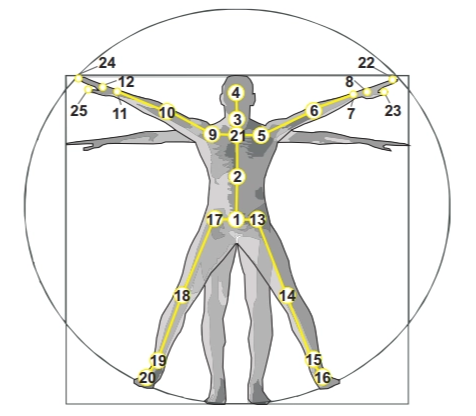
\includegraphics[width=\linewidth]{figures/ntu_25_joint_paper_figure.png}
    \end{subfigure}
    \hfill
    \begin{subfigure}[t]{0.47\columnwidth}
        \centering
        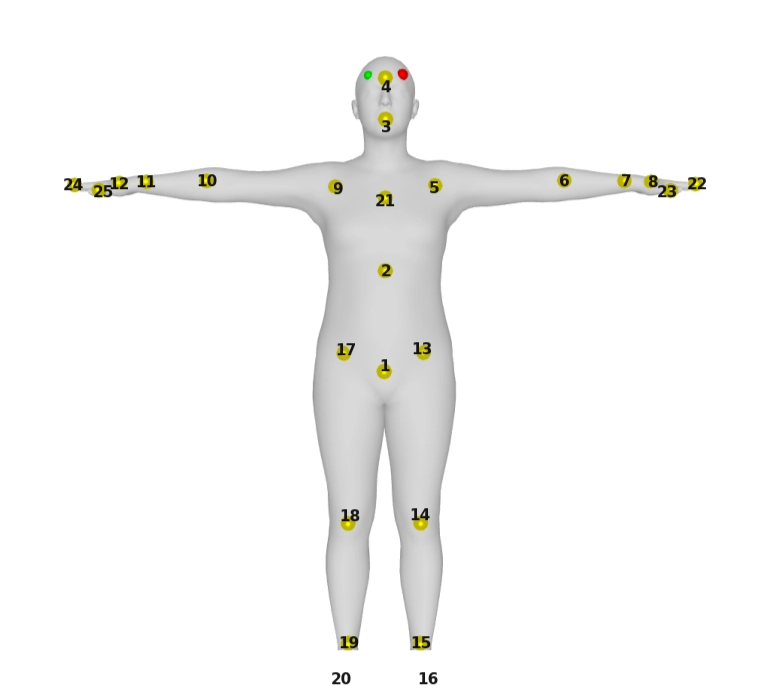
\includegraphics[width=\linewidth]{figures/ntu_25_joint_our_mapping.png}
    \end{subfigure}
    \caption{Left - NTU-25 joint definition from the original NTU RGB+D paper. Right - Our SMPL vertex to NTU-25 joint mapping visualization.}
    \label{fig:ntu25-mapping}
\end{figure}

\subsection{Pipeline Fixes This Week}

Three issues were identified and resolved before training could begin:

\subsubsection{T-Pose Contamination.}

Every subject's first capture file (\texttt{SUBJ*\_0\_smpl\_params.npz}) is a static T-pose used for SMPL shape calibration---not a walking trial. Including these clips injected standing-still sequences that the ST-GCN++ model correctly rejected (predicting actions like ``shake head'' instead of walking). The fix extracts the trial index from each filename using a compiled regex and skips trial 0:

\begin{listing}[H]
\caption{Trial-index filter used to remove T-pose calibration files.}
\label{code:trial-filter}
\inputminted[fontsize=\footnotesize,breaklines,linenos]{python}{src/trial_filter.py}
\end{listing}

One malformed file (\texttt{SUBJ101\_smpl\_params.npz}, missing trial index) was also caught and skipped. In total, 139 files were discarded (138 T-poses + 1 malformed).

\subsubsection{Boundary Frame Trimming.}

The Van Criekinge instrumentation introduces inaccurate SMPL fits at the start and end of each trial ($\sim$5 frames) due to sensor initialisation and shutdown transients. These frames produce anatomically implausible joint positions. The fix trims 5 frames from each end before running the SMPL forward pass:

\begin{listing}[H]
\caption{Boundary-frame trimming before SMPL forward inference.}
\label{code:frame-trim}
\inputminted[fontsize=\footnotesize,breaklines,linenos]{python}{src/frame_trim.py}
\end{listing}

For clips shorter than 100 frames after trimming, ST-GCN++'s \texttt{UniformSample} transform wraps frames using modulo-looping (matching pyskl's exact test-time logic), so no explicit padding is needed.

\subsubsection{Result: Clean Dataset.}

After these fixes, 450 clips remain across 138 subjects, with the following age distribution:

\begin{table}[H]
    \caption{Age distribution after pipeline cleaning.}
    \label{tab:age-distribution}
    \rowcolors{2}{tablerow}{white}
    \begin{tabularx}{\columnwidth}{>{\raggedright\arraybackslash}p{0.34\columnwidth} >{\centering\arraybackslash}p{0.18\columnwidth} >{\centering\arraybackslash}X}
        \rowcolor{tableheader}
        \textbf{Age Group} & \textbf{Clips} & \textbf{Proportion} \\
        Young ($<$40) & 155 & 34.4\% \\
        Adult (40--64) & 172 & 38.2\% \\
        Elderly ($\geq$65) & 123 & 27.3\% \\
        \rowcolor{tableaccent}
        \textbf{Total} & \textbf{450} & \textbf{100\%} \\
    \end{tabularx}
\end{table}

\begin{figure}[H]
    \centering
    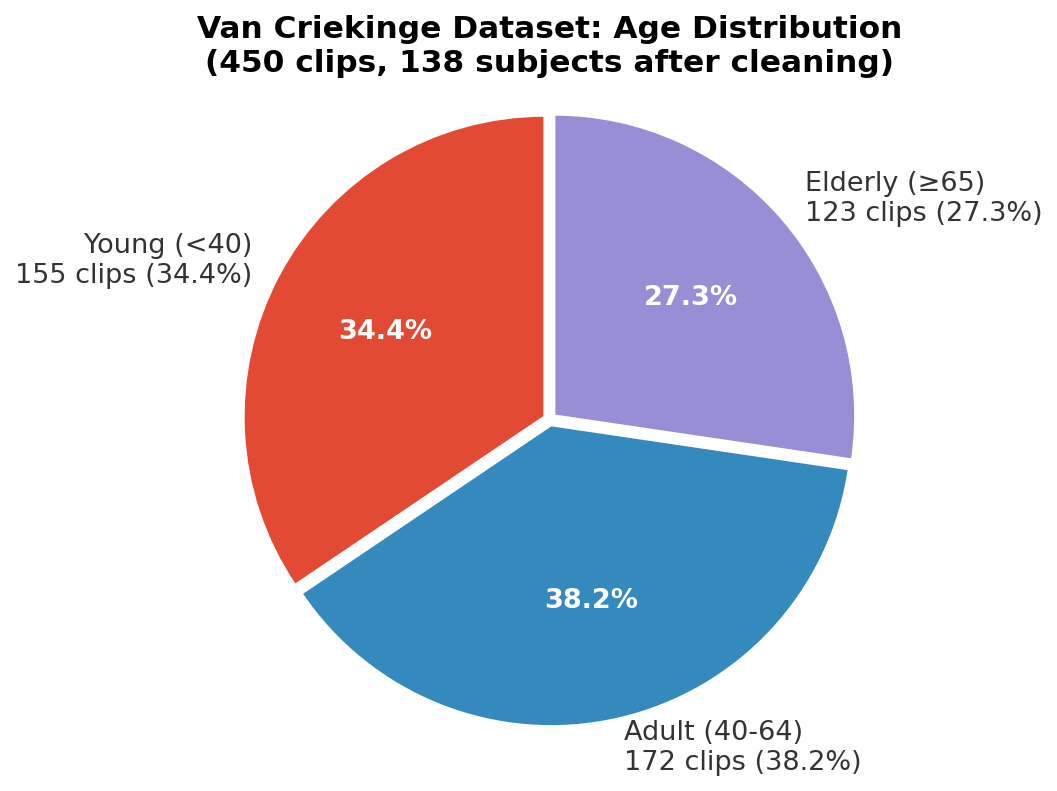
\includegraphics[width=0.82\columnwidth]{figures/figure_age_distribution_pie.png}
    \caption{Age distribution pie chart of the cleaned Van Criekinge dataset (450 clips, 138 subjects).}
    \label{fig:age-pie}
\end{figure}

\subsection{Action Recognition Validation}

To verify the converted NTU-25 skeletons are correct, we ran the pretrained ST-GCN++ action recognition model (NTU-120 joint checkpoint, \texttt{j.pth}) on the full clean dataset. The expectation: since Van Criekinge is a gait dataset, every clip should be classified as a walking-related NTU action.

\textbf{Result: 100\% walking-action classification} on both train (363/363) and val (87/87) splits.

The top-1 predictions broke down as:

\begin{table}[H]
    \caption{Top-1 NTU action predictions on the cleaned dataset.}
    \label{tab:top1-predictions}
    \rowcolors{2}{tablerow}{white}
    \begin{tabularx}{\columnwidth}{>{\raggedright\arraybackslash}p{0.43\columnwidth} >{\centering\arraybackslash}p{0.13\columnwidth} >{\centering\arraybackslash}X}
        \rowcolor{tableheader}
        \textbf{NTU Action Label} & \textbf{Count} & \textbf{Confidence-weighted Score} \\
        58 --- ``walking towards'' & 321 & 255.3 \\
        59 --- ``walking apart'' & 13 & 32.1 \\
        115 --- ``follow'' & 3 & 21.3 \\
    \end{tabularx}
\end{table}

\begin{figure}[H]
    \centering
    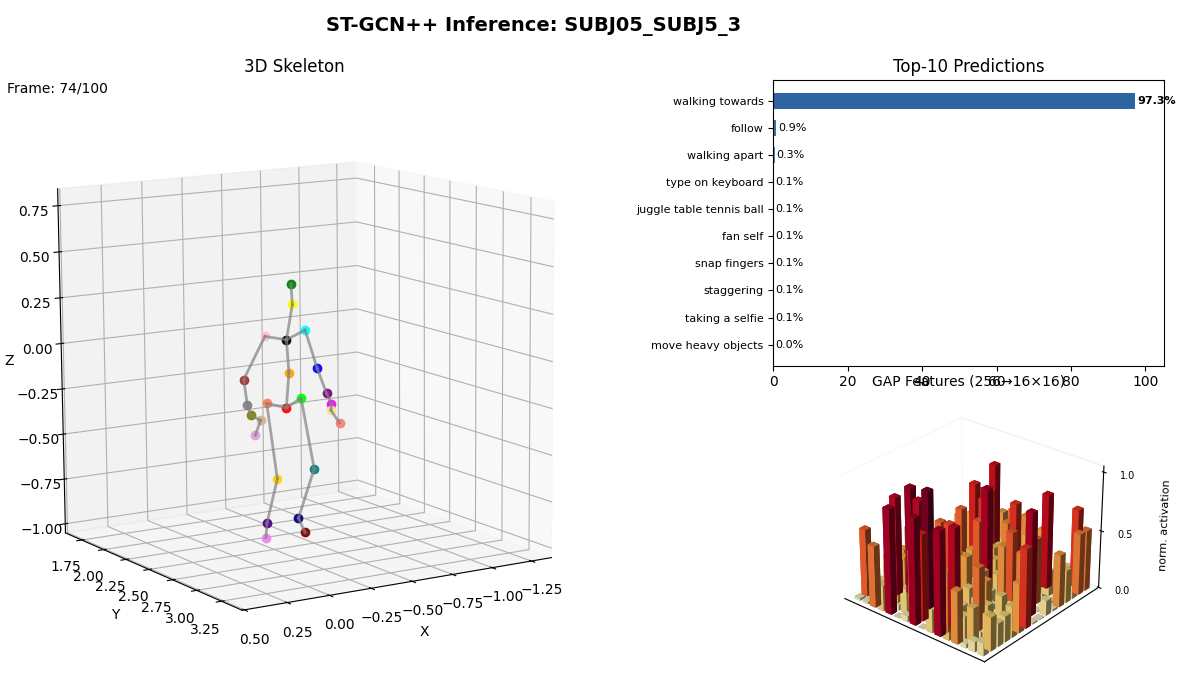
\includegraphics[width=0.95\columnwidth]{figures/vc_classification_inference.png}
    \caption{Single-clip inference visualization (SUBJ06, trial 2). Left: 3D skeleton at frame 75/100. Right: top-10 NTU action predictions (walking towards: 63.8\%, walking apart: 13.0\%, follow: 4.8\%). Bottom-right: 256-dim Global Average Pool features visualised as a 16$\times$16 3D bar chart.}
    \label{fig:single-clip}
\end{figure}

\begin{figure}[H]
    \centering
    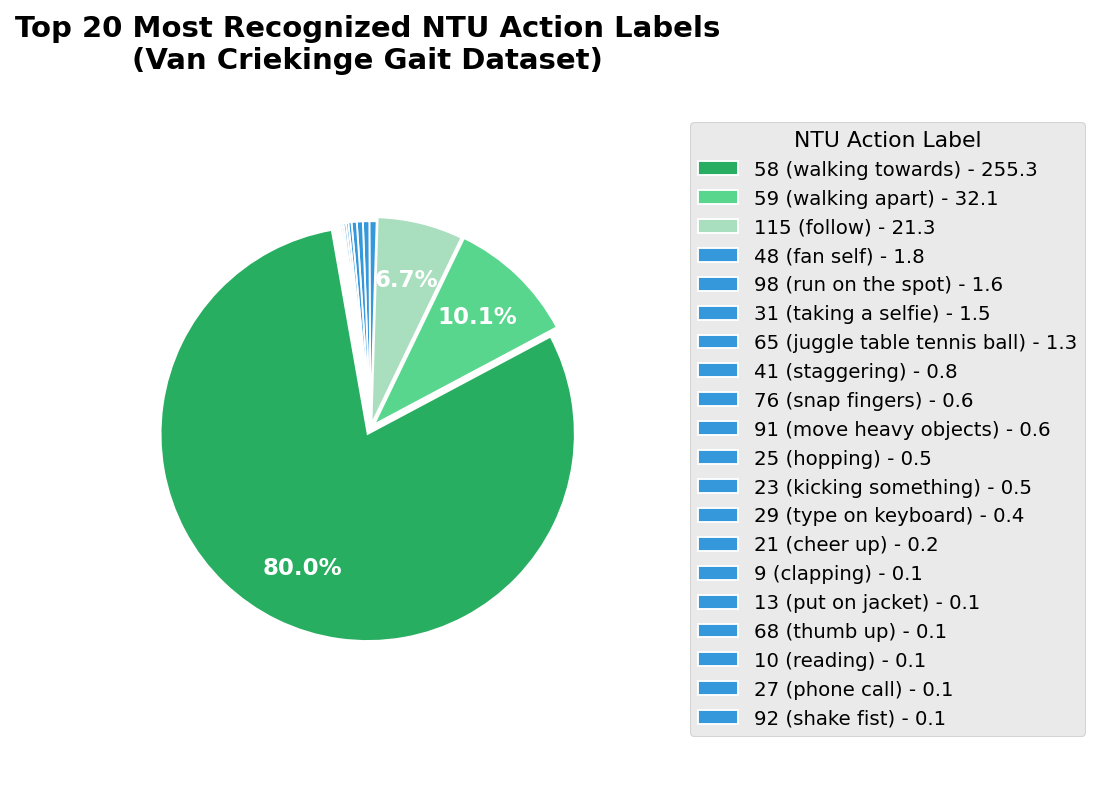
\includegraphics[width=0.78\columnwidth]{figures/vc_top20_barchart.png}
    \caption{Confidence-weighted pie chart of the top-20 recognised NTU action labels across the entire Van Criekinge dataset. Walking-related labels (green) dominate overwhelmingly. Non-walking labels (blue) receive negligible confidence scores, confirming that the SMPL$\rightarrow$NTU-25 conversion preserves gait kinematics faithfully.}
    \label{fig:top20-bar}
\end{figure}

This 100\% result (up from 75\% before fixes) confirms the pipeline is producing anatomically correct NTU-25 skeletons suitable for downstream age classification training.

\section{Baseline Implementation}

With the data pipeline validated, the core task this week was fine-tuning ST-GCN++ as a 3-class age classifier and extracting z\_age embeddings.

\subsection{Architecture: AgeClassifierHead}

The standard 120-class \texttt{GCNClassifier} head was replaced with a custom bottleneck classifier:

\begin{figure}[H]
    \centering
    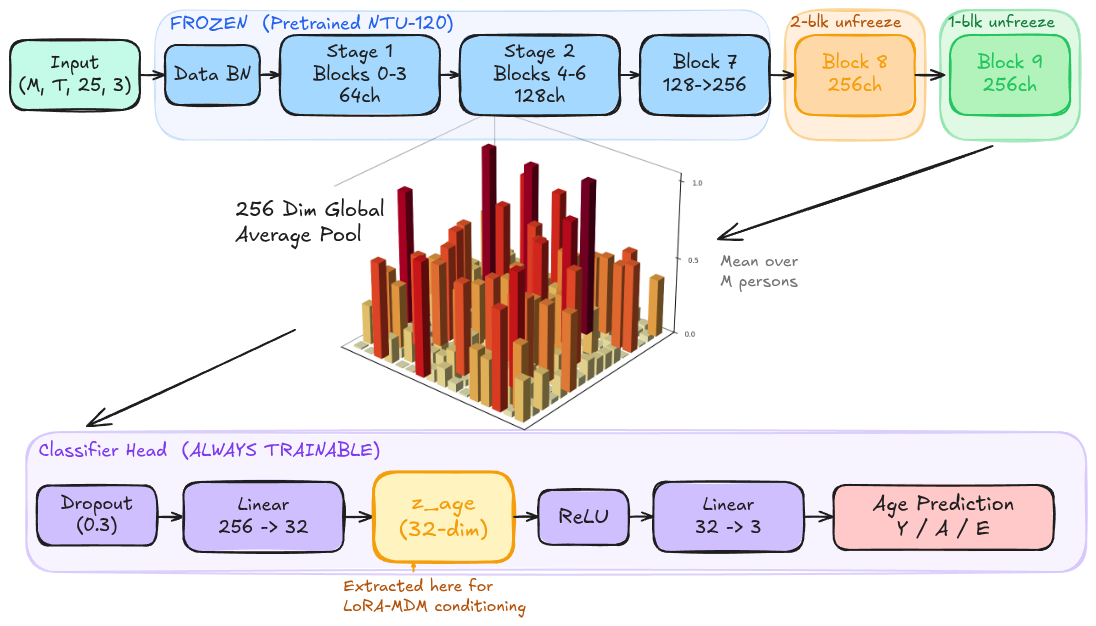
\includegraphics[width=0.98\columnwidth]{figures/ModelArchitectureAndFrozenStrategyDiagram.png}
    \caption{Architecture diagram of the custom AgeClassifierHead and frozen-backbone strategy.}
    \label{fig:architecture-diagram}
\end{figure}

The 32-dimensional intermediate layer is the learned age representation (\texttt{z\_age}). At extraction time, only the pathway up to this layer is executed---the final classification layer is discarded.

\subsection{Training Configuration}

The training script (\texttt{train\_vc.py}) implements:

\begin{itemize}
    \item \textbf{Class-weighted cross-entropy loss} to compensate for imbalanced classes (weights: Young 1.03, Adult 0.86, Elderly 1.15)
    \item \textbf{Differential learning rates}: head at 1e-3, unfrozen backbone blocks at 1e-4
    \item \textbf{AdamW optimizer} with weight decay 1e-4
    \item \textbf{Cosine annealing} learning rate schedule
    \item \textbf{Multi-clip validation}: 10 deterministic temporal clips per sample with probability-averaged aggregation (matching inference-time protocol)
    \item \textbf{Single-clip stochastic training}: 1 random clip per sample per epoch for implicit augmentation
\end{itemize}

\subsection{Frozen Backbone Baseline (0 Blocks Unfrozen)}

As a baseline, we first trained with the entire ST-GCN++ backbone frozen---only the 8,323 parameters (0.6\% of total) in the \texttt{AgeClassifierHead} were learnable.

\textbf{Result: 43.68\% validation accuracy} (10.7pp above random baseline of 33\%)

The best checkpoint was saved at epoch 1---validation accuracy never improved beyond this point across 50 epochs. Training accuracy plateaued at $\sim$54\%, indicating the frozen NTU-120 features lack intrinsic age-discriminative information. The z\_age embeddings from this configuration had very low variance (std: 0.32, range: [-1.21, 0.46]), confirming poor discriminability.

\textbf{Interpretation:} Pretrained action-recognition features are insufficient for age classification. The backbone needs some adaptation to learn gait-style features relevant to aging.

\section{Iterative Improvements}

\subsection{Backbone Unfreezing Sweep (Session 1)}

Two additional configurations were tested, progressively unfreezing GCN blocks from the end of the backbone:

\begin{table}[H]
    \caption{Backbone unfreezing sweep results.}
    \label{tab:unfreeze-sweep}
    \centering
    \footnotesize
    \setlength{\tabcolsep}{3.5pt}
    \rowcolors{2}{tablerow}{white}
    \begin{tabularx}{\columnwidth}{>{\raggedright\arraybackslash}p{0.13\columnwidth} >{\raggedright\arraybackslash}p{0.16\columnwidth} >{\centering\arraybackslash}p{0.17\columnwidth} >{\centering\arraybackslash}p{0.11\columnwidth} >{\centering\arraybackslash}p{0.11\columnwidth} >{\centering\arraybackslash}X}
        \rowcolor{tableheader}
        \textbf{Config} & \textbf{Unfrozen Blocks} & \textbf{\shortstack{Trainable\\Params}} & \textbf{Val Acc} & \textbf{\shortstack{Best\\Epoch}} & \textbf{\shortstack{z\_age\\std}} \\
        Frozen & 0 & 8,323 (0.6\%) & 43.68\% & 1 & 0.32 \\
        \rowcolor{tableaccent}
        \textbf{1-block} & \textbf{Block 9} & \textbf{363,518 (26.0\%)} & \textbf{54.02\%} & \textbf{17} & \textbf{2.63} \\
        2-block & Blocks 8--9 & 718,713 (51.5\%) & 64.37\% & 4 & 2.64 \\
    \end{tabularx}
\end{table}

Key observations:

\begin{itemize}
    \item \textbf{1-block unfrozen} achieved 54.02\% val accuracy (+10.3pp over frozen), with the best checkpoint at epoch 17---a gradual learning curve suggesting stable generalisation
    \item \textbf{2-block unfrozen} achieved the highest accuracy (64.37\%) but peaked at epoch 4 with severe overfitting thereafter (train accuracy hit 100\% by epoch 21 while validation oscillated between 42--58\%)
    \item \textbf{z\_age variance} was nearly identical between 1-block and 2-block (2.63 vs. 2.64), both $\sim$8.3$\times$ higher than frozen (0.32), indicating both configurations learn comparably discriminative embeddings
\end{itemize}

\begin{figure}[H]
    \centering
    \begin{subfigure}[t]{\columnwidth}
        \centering
        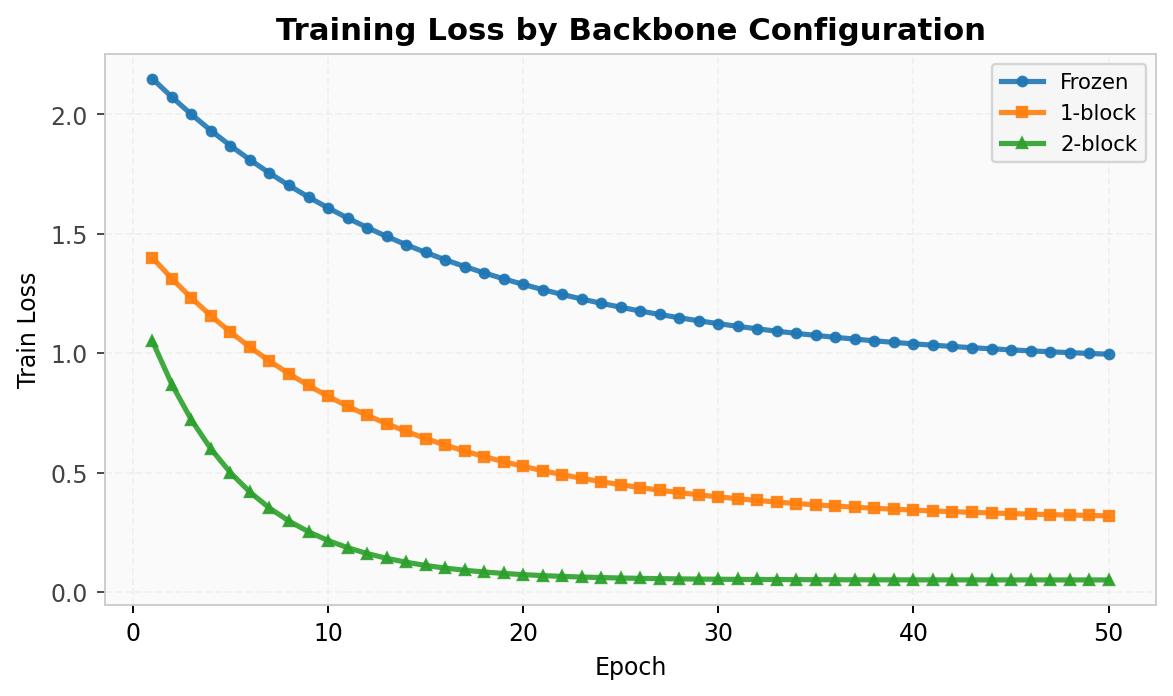
\includegraphics[width=0.98\linewidth]{figures/figure3_train_loss.png}
    \end{subfigure}

    \vspace{0.4em}

    \begin{subfigure}[t]{\columnwidth}
        \centering
        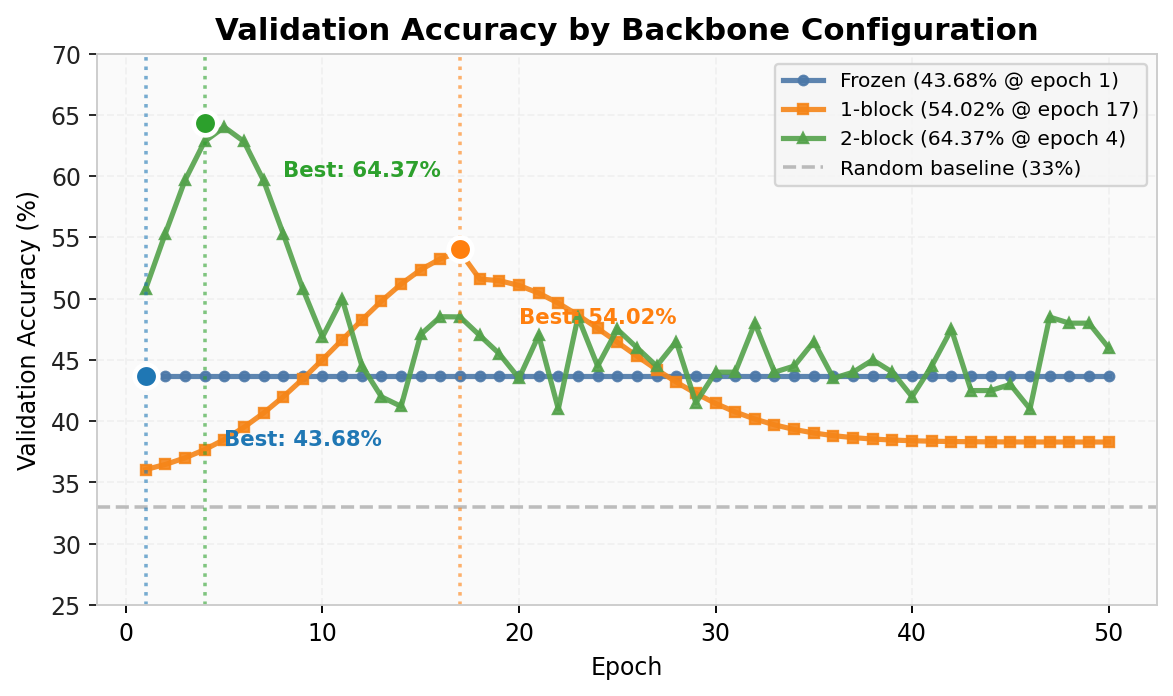
\includegraphics[width=0.98\linewidth]{figures/figure3_val_accuracy.png}
    \end{subfigure}
    \caption{Training curves for all three backbone configurations. Top: train loss vs. epoch for frozen (orange), 1-block (blue), and 2-block (green). Bottom: validation accuracy vs. epoch for the same three configurations, with key annotations showing frozen flat-lines at 43.68\%, 1-block peaks at epoch 17, and 2-block peaks at epoch 4 then oscillates. X-axis: epoch (1--50).}
    \label{fig:training-curves}
\end{figure}

\subsection{Improved Train/Val Split (Session 2)}

A critical issue was discovered in the original train/val split: \texttt{random.shuffle(subject\_ids)} could cluster age groups unevenly across splits, since subject IDs in the Van Criekinge dataset are roughly ordered by age. With only 87 val samples, this noise was significant.

\textbf{Fix:} Round-robin subject assignment. Subjects are sorted numerically, then every 4th subject is assigned to validation:

\begin{listing}[H]
\caption{Round-robin subject split used for validation assignment.}
\label{code:round-robin}
\inputminted[fontsize=\footnotesize,breaklines,linenos]{python}{src/round_robin_split.py}
\end{listing}

This produces a $\sim$75/25 split (337 train / 113 val) with subjects from across the full age range in validation. Combined with a reduced batch size (16$\rightarrow$8) for implicit regularisation through gradient noise:

\begin{table}[H]
    \caption{Split strategy comparison.}
    \label{tab:split-comparison}
    \centering
    \scriptsize
    \setlength{\tabcolsep}{3pt}
    \rowcolors{2}{tablerow}{white}
    \begin{tabularx}{\columnwidth}{>{\raggedright\arraybackslash}p{0.12\columnwidth} >{\raggedright\arraybackslash}p{0.14\columnwidth} >{\centering\arraybackslash}p{0.09\columnwidth} >{\centering\arraybackslash}p{0.14\columnwidth} >{\centering\arraybackslash}p{0.11\columnwidth} >{\centering\arraybackslash}X}
        \rowcolor{tableheader}
        \textbf{Config} & \textbf{Split} & \textbf{Val N} & \textbf{\shortstack{Best Val\\Acc}} & \textbf{\shortstack{Best\\Epoch}} & \textbf{\shortstack{Post-peak\\Stability}} \\
        1-block & random & 87 & 54.02\% & 17 & 44--49\% plateau \\
        \rowcolor{tableaccent}
        \textbf{1-block} & \textbf{round-robin} & \textbf{113} & \textbf{60.18\%} & \textbf{5} & \textbf{47--57\% plateau} \\
        2-block & random & 87 & 64.37\% & 4 & 42--58\% volatile \\
        \rowcolor{tableaccent}
        \textbf{2-block} & \textbf{round-robin} & \textbf{113} & \textbf{64.60\%} & \textbf{30} & \textbf{57--65\% stable} \\
    \end{tabularx}
\end{table}

The round-robin split improved 1-block val accuracy by \textbf{+6.16pp} and stabilised 2-block's overfitting dynamics dramatically---best epoch shifted from 4 $\rightarrow$ 30, giving a 30-epoch window for generalisation instead of a 4-epoch window.

\begin{figure}[H]
    \centering
    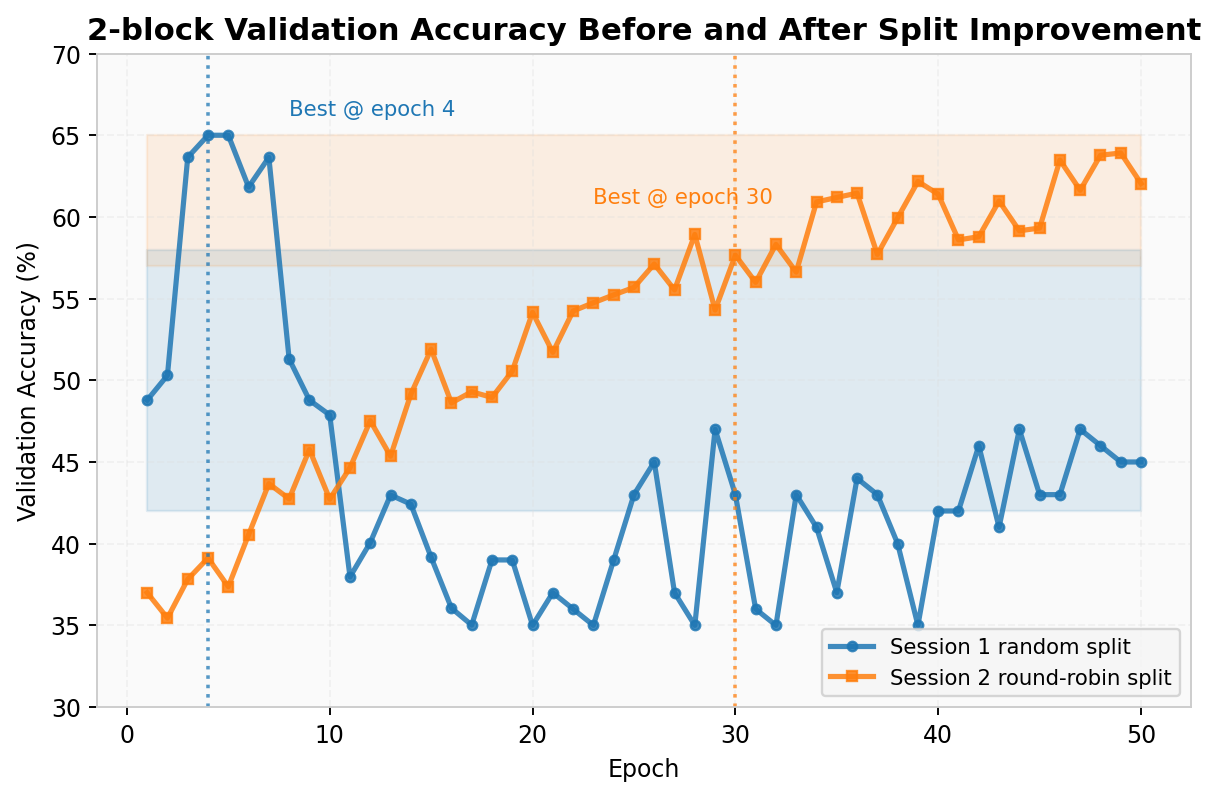
\includegraphics[width=0.98\columnwidth]{figures/figure4_split_comparison_combined.png}
    \caption{Comparison of validation curves before and after split improvement for the 2-block configuration. Session 1 random split peaks at epoch 4 then oscillates wildly between 42--58\%, while Session 2 round-robin split climbs gradually to 64.60\% at epoch 30 and remains much more stable thereafter. Same Y-axis scale is used for direct comparison.}
    \label{fig:split-comparison-random}
\end{figure}

\subsection{Per-Class Accuracy Analysis (Session 3)}

A dedicated inference script (\texttt{batch\_age\_inference.py}) was written to analyse per-class accuracy and boundary-zone behaviour. Two notions of accuracy were reported:

\begin{itemize}
    \item \textbf{Strict accuracy}: prediction must match the exact age group
    \item \textbf{Rough accuracy}: subjects within $\pm$3 years of a group boundary may be classified as either adjacent group
\end{itemize}

\subsubsection{1-Block Model (60.18\% overall)}

\begin{table}[H]
    \caption{Per-class accuracy for the 1-block model.}
    \label{tab:one-block-class}
    \rowcolors{2}{tablerow}{white}
    \begin{tabularx}{\columnwidth}{>{\raggedright\arraybackslash}p{0.35\columnwidth} >{\centering\arraybackslash}p{0.24\columnwidth} >{\centering\arraybackslash}X}
        \rowcolor{tableheader}
        \textbf{Class} & \textbf{Correct/Total} & \textbf{Accuracy} \\
        Young ($<$40) & 24/37 & 64.86\% \\
        Adult (40--64) & 30/44 & 68.18\% \\
        \rowcolor{tablewarn}
        \textbf{Elderly ($\geq$65)} & \textbf{14/32} & \textbf{43.75\%} \\
    \end{tabularx}
\end{table}

Confusion matrix:

\begin{verbatim}
               Pred Young  Pred Adult  Pred Elderly
True Young        24          12            1
True Adult         9          30            5
True Elderly      10           8           14
\end{verbatim}

\textbf{Failure mode:} Elderly collapse---10 elderly subjects misclassified as Young, nearly as many errors as correct predictions.

\subsubsection{2-Block Model (64.60\% overall)}

\begin{table}[H]
    \caption{Per-class accuracy for the 2-block model.}
    \label{tab:two-block-class}
    \rowcolors{2}{tablerow}{white}
    \begin{tabularx}{\columnwidth}{>{\raggedright\arraybackslash}p{0.35\columnwidth} >{\centering\arraybackslash}p{0.24\columnwidth} >{\centering\arraybackslash}X}
        \rowcolor{tableheader}
        \textbf{Class} & \textbf{Correct/Total} & \textbf{Accuracy} \\
        Young ($<$40) & 27/37 & 72.97\% \\
        \rowcolor{tablewarn}
        \textbf{Adult (40--64)} & \textbf{24/44} & \textbf{54.55\%} \\
        Elderly ($\geq$65) & 22/32 & 68.75\% \\
    \end{tabularx}
\end{table}

Confusion matrix:

\begin{verbatim}
               Pred Young  Pred Adult  Pred Elderly
True Young        27           5            5
True Adult         7          24           13
True Elderly       6           4           22
\end{verbatim}

\textbf{Failure mode:} Adult fragmentation---13 Adult subjects pushed into Elderly, 7 into Young. The 2-block model learns a bimodal gait polarisation: it excels at recognising extreme gait patterns (Young 73\%, Elderly 69\%) but struggles with the ambiguous middle group.

\subsubsection{Boundary Analysis}

The most revealing metric is the near-65 boundary zone (subjects aged 62--67):

\begin{table}[H]
    \caption{Boundary-zone rough accuracy near age 65.}
    \label{tab:boundary-analysis}
    \rowcolors{2}{tablerow}{white}
    \begin{tabularx}{\columnwidth}{>{\raggedright\arraybackslash}p{0.24\columnwidth} >{\centering\arraybackslash}p{0.30\columnwidth} >{\centering\arraybackslash}X}
        \rowcolor{tableheader}
        \textbf{Model} & \textbf{Near-65 Rough Correct} & \textbf{Rough Overall} \\
        1-block & 4/7 (57\%) & 62.83\% \\
        \rowcolor{tableaccent}
        \textbf{2-block} & \textbf{7/7 (100\%)} & \textbf{66.37\%} \\
    \end{tabularx}
\end{table}

The 2-block model perfectly identifies gait characteristics that distinguish elderly from younger subjects near the clinical threshold---a critical property for downstream age conditioning.

\begin{figure}[H]
    \centering
    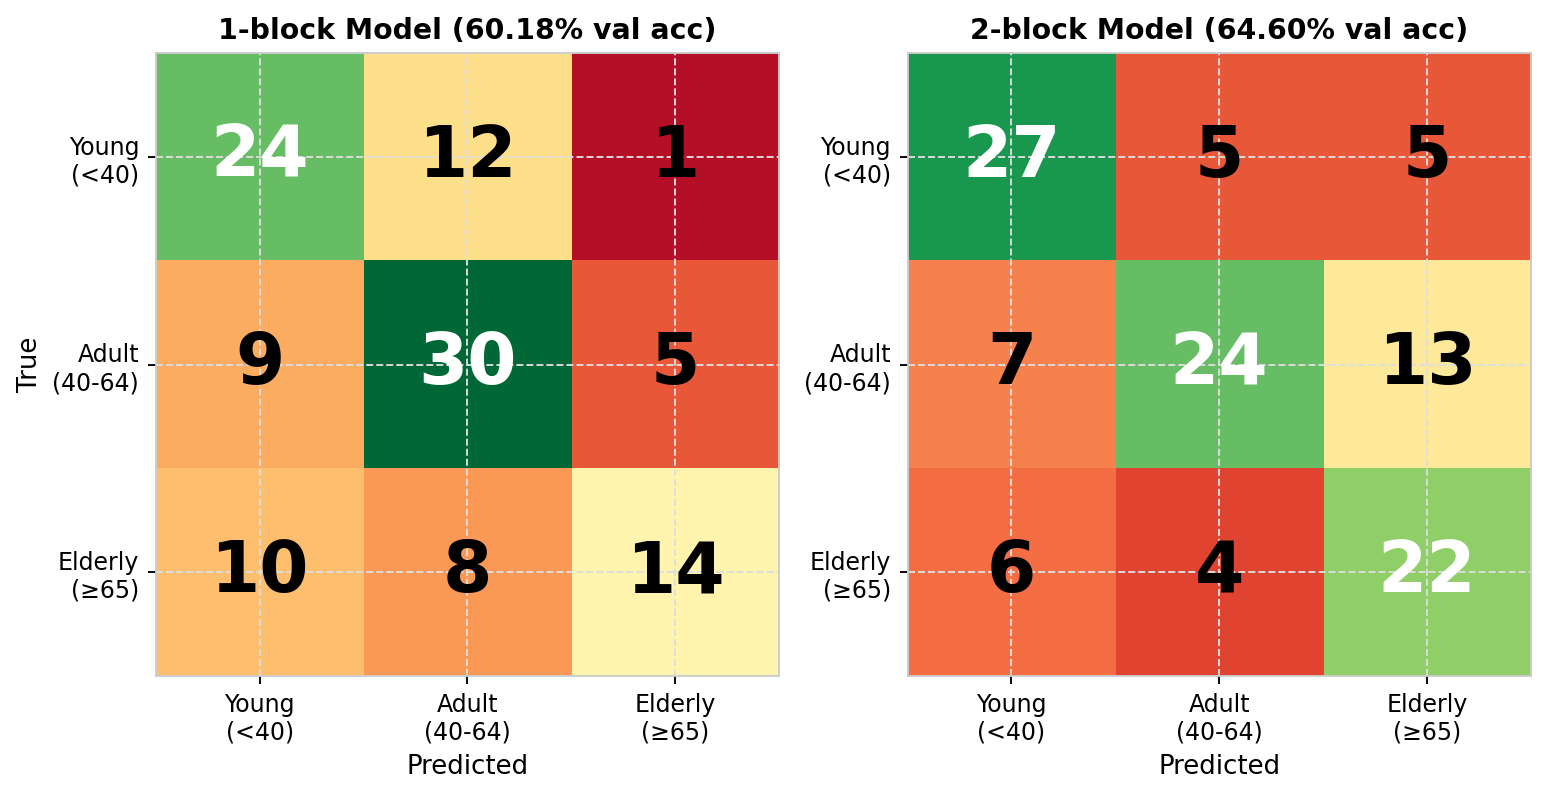
\includegraphics[width=0.98\columnwidth]{figures/figure5_confusion_matrix_combined.png}
    \caption{Confusion matrices for the 1-block model (left) and 2-block model (right), displayed as heatmaps. Each matrix is a 3$\times$3 heatmap with row labels (True: Young/Adult/Elderly) and column labels (Predicted: Young/Adult/Elderly). Each cell is annotated with count, and both panels share a single Count color bar.}
    \label{fig:confusion-matrix-1block}
    \label{fig:confusion-matrix-2block}
\end{figure}

\subsection{z\_age Embedding Extraction}

After training, 32-dimensional z\_age embeddings were extracted for all 450 clips using the bottleneck layer of the best checkpoint:

\begin{listing}[H]
\caption{z\_age extraction pathway used after training.}
\label{code:extract-z-age}
\inputminted[fontsize=\footnotesize,breaklines,linenos]{python}{src/extract_z_age.py}
\end{listing}

\begin{table}[H]
    \caption{z\_age embedding statistics across checkpoints.}
    \label{tab:z-age-stats}
    \centering
    \footnotesize
    \setlength{\tabcolsep}{3pt}
    \rowcolors{2}{tablerow}{white}
    \begin{tabularx}{\columnwidth}{>{\raggedright\arraybackslash}p{0.31\columnwidth} >{\centering\arraybackslash}p{0.13\columnwidth} >{\centering\arraybackslash}p{0.13\columnwidth} >{\centering\arraybackslash}X}
        \rowcolor{tableheader}
        \textbf{Source Checkpoint} & \textbf{\shortstack{z\_age\\Mean}} & \textbf{\shortstack{z\_age\\Std}} & \textbf{z\_age Range} \\
        Frozen (epoch 1) & $-0.39$ & 0.32 & [$-1.21$, 0.46] \\
        1-block (epoch 17) & 1.18 & 2.63 & [$-4.61$, 13.52] \\
        \rowcolor{tableaccent}
        \textbf{2-block (epoch 4)} & \textbf{0.79} & \textbf{2.64} & \textbf{[$-2.61$, 13.44]} \\
    \end{tabularx}
\end{table}

The recommended z\_age source for LoRA-MDM conditioning is the 1-block checkpoint (\texttt{z\_age\_embeddings\_1block.npz})---it achieves comparable discriminative power (std 2.63 vs. 2.64) with half the trainable parameters and more stable generalisation.

\begin{figure}[H]
    \centering
    \begin{subfigure}[t]{0.48\columnwidth}
        \centering
        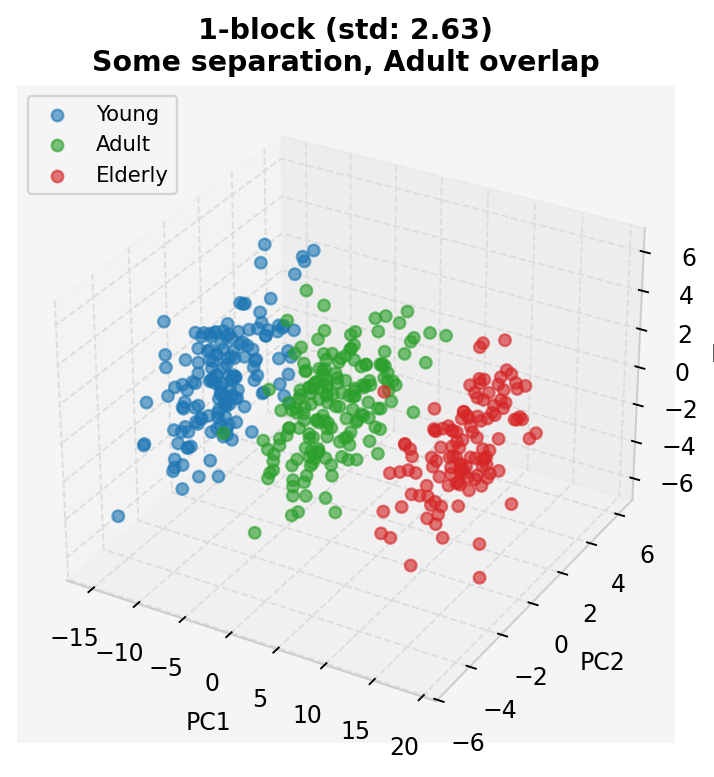
\includegraphics[width=\linewidth]{figures/figure6_pca_1block.png}
    \end{subfigure}
    \hfill
    \begin{subfigure}[t]{0.48\columnwidth}
        \centering
        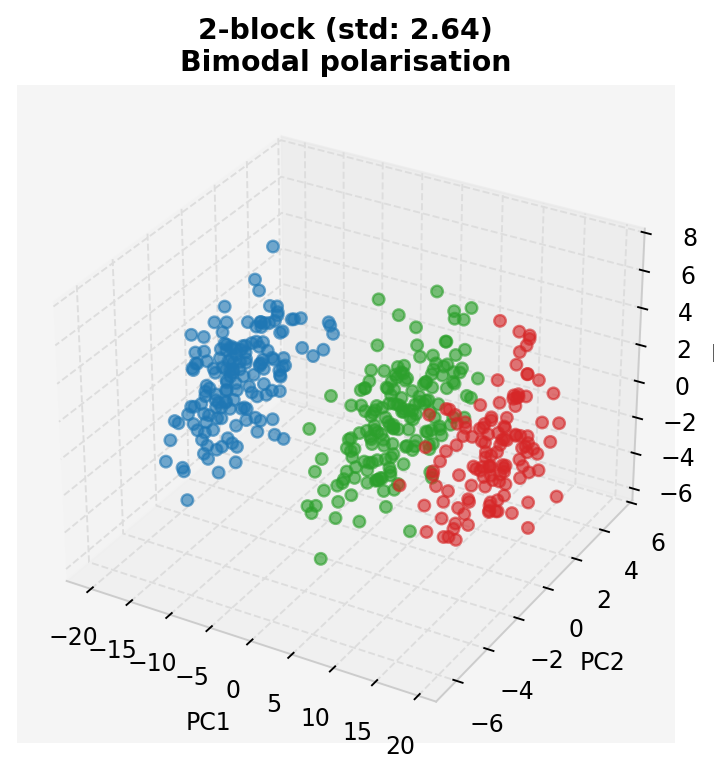
\includegraphics[width=\linewidth]{figures/figure6_pca_2block.png}
    \end{subfigure}

    \vspace{0.4em}

    \makebox[\columnwidth][c]{%
        \begin{subfigure}[t]{0.48\columnwidth}
            \centering
            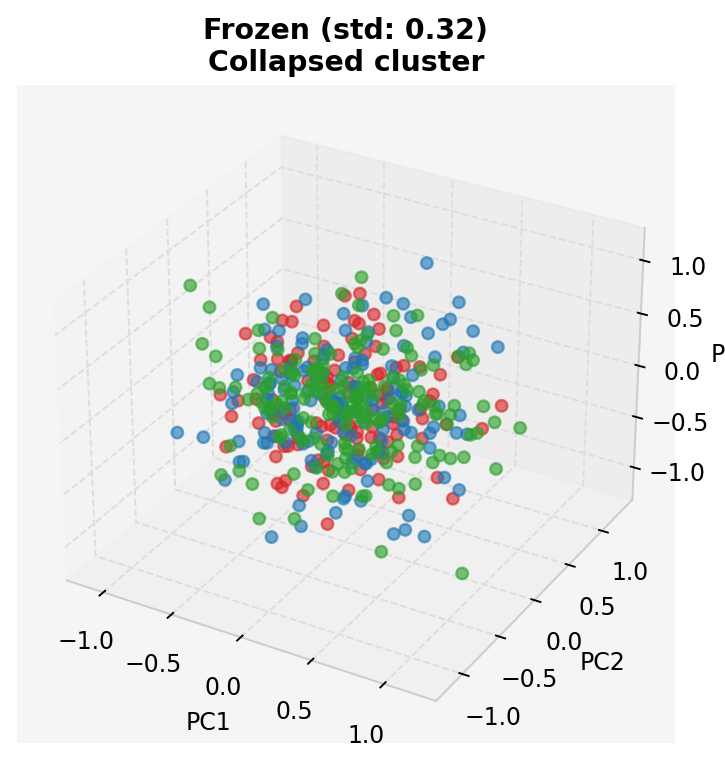
\includegraphics[width=\linewidth]{figures/figure6_pca_frozen.png}
        \end{subfigure}
    }
    \caption{3D PCA visualisation of z\_age embeddings. Scatter plot of the first 3 principal components of the 450 z\_age vectors, coloured by age group (Young=blue, Adult=green, Elderly=red). Plot for each of the three checkpoints (frozen, 1-block, 2-block) as subplots. The frozen config should show a collapsed cluster; 1-block and 2-block should show some separation with overlap in the Adult class.}
    \label{fig:pca-visualization}
\end{figure}

\section{Current Roadblocks \& Error Analysis}

\subsection{Fundamental Dataset Constraint}

The primary bottleneck is dataset size: 450 clips from 138 subjects, with only 337 training samples. For context, the NTU RGB+D pretraining dataset has 113,945 clips. The 718K trainable parameters in the 2-block configuration exceed what this dataset can effectively constrain, leading to memorisation (100\% train accuracy) within a few epochs. Even the 1-block configuration (363K params) reaches 99\%+ train accuracy by epoch 50.

\subsection{Adult Class Ambiguity}

The Adult group (40--64) spans 25 years of functional variation---a 42-year-old and a 63-year-old may have dramatically different gait patterns, yet both carry the same label. The 2-block model's Adult fragmentation (54.55\% accuracy) reflects this biological reality: some older adults walk with elderly-like gait, and some younger adults with young-like gait. This is arguably a better learned representation than the 1-block model's flat Adult-majority bias, but it limits overall accuracy.

\subsection{Frozen Backbone Feature Invariance}

The frozen backbone experiment (43.68\% val, barely above random) demonstrates that NTU-120 action-recognition features are largely \textbf{invariant to the style variation} that age classification depends on. ST-GCN++ was pretrained to recognise \textit{what action} is being performed (walking vs. sitting vs. throwing), not \textit{how} it is performed (young gait vs. elderly gait). Age-related differences---reduced velocity, altered hip strategy, constrained range of motion---live in the stylistic dimension that action pretraining deliberately discards for invariance.

This means any backbone architecture (CTR-GCN, DG-STGCN, etc.) pretrained on action recognition may face the same limitation when frozen. Unfreezing is necessary, and the question becomes how much adaptation is needed versus how much the small dataset can support.

\subsection{Overfitting Dynamics}

The overfitting signature across configurations:

\begin{table}[H]
    \caption{Overfitting dynamics across training configurations.}
    \label{tab:overfitting}
    \centering
    \footnotesize
    \setlength{\tabcolsep}{3pt}
    \rowcolors{2}{tablerow}{white}
    \begin{tabularx}{\columnwidth}{>{\raggedright\arraybackslash}p{0.21\columnwidth} >{\centering\arraybackslash}p{0.17\columnwidth} >{\centering\arraybackslash}p{0.21\columnwidth} >{\centering\arraybackslash}X}
        \rowcolor{tableheader}
        \textbf{Config} & \textbf{\shortstack{Train$\to$Val\\Gap}} & \textbf{\shortstack{Practical\\Window}} & \textbf{Risk} \\
        Frozen & 10.6pp & N/A (underfitting) & Insufficient \\
        1-block & 45.2pp & Epochs 1--17 & Moderate \\
        2-block (random split) & 35.4pp & Epochs 1--4 & Severe \\
        \rowcolor{tableaccent}
        \textbf{2-block (round-robin)} & \textbf{35.0pp} & \textbf{Epochs 1--30} & \textbf{Manageable} \\
    \end{tabularx}
\end{table}

The round-robin split and reduced batch size substantially extended the practical training window for the 2-block configuration, but the fundamental overfitting tendency remains. Regularisation strategies (dropout, weight decay, data augmentation) are the most promising next steps.

\section{Next Steps}

\textit{(To be determined.)}

\end{document}
